%%%% Document setup
\documentclass[a4paper,landscape,title page]{article}
\setlength{\oddsidemargin}{-0.65in}	% default=0in
\setlength{\textwidth}{11in}		% default=9in
\setlength{\textheight}{6.85in}		% default=5.15in
\setlength{\topmargin}{-1.0in}		% default=0.20in
\setlength{\headsep}{0.35in}		% default=0.35in
\setlength{\parskip}{1.2ex}
\setlength{\parindent}{0mm}

%%%% Use packages
\usepackage{times}
\usepackage{tikz,pgf}
\usetikzlibrary{arrows,automata,trees,plotmarks,calc}


%%%%
\title{Goal-Plan hierarchy for test \textit{testfr01}}
\author{
Dhirendra Singh\\
dhirendra.singh@rmit.edu.au}
\begin{document}
\maketitle

\begin{figure*}[t]
\begin{center}

\begin{tikzpicture}[scale=1.1,level distance=1.4cm]
\tikzstyle{txt}=[scale=1.1]
\tikzstyle{planbox}=[scale=1.1,draw,minimum height=0.7cm,minimum width=1.1cm]
\tikzstyle{goalbox}=[scale=1.1,draw,rounded corners,minimum height=0.7cm,minimum width=1.1cm]
\tikzstyle{level 1}=[sibling distance=8.0cm] 
\tikzstyle{level 2}=[sibling distance=6.0cm] 
\tikzstyle{level 3}=[sibling distance=3.0cm]
\tikzstyle{level 4}=[sibling distance=3.0cm]
\tikzstyle{level 5}=[sibling distance=1.5cm]
\tikzstyle{level 6}=[sibling distance=3.0cm]
\tikzstyle{level 7}=[sibling distance=1.5cm]

\node[goalbox,yshift=1cm,solid] (T) {$G$}
	child[dashed] {node[planbox] (xP) {$xP$}}
	child[solid] {node[planbox] (yP) {$yP$}
		child {node[goalbox] {$yG_{a}$}
			child {node[planbox] {$yP_{a1}$}
				child {node[goalbox] {$yG_{aa}$}
					child {node[planbox] {$yP_{aa1}$}
						child {node[goalbox] {$yG_{aaa}$}
							child {node[planbox] {$yP_{aaa1}$} node[txt,below=0.3cm] {$\surd$}}
							child {node[planbox] {$yP_{aaa*}$} node[txt,below=0.3cm] {$\times$}
								edge from parent node[txt,right,near start] {$\times 3$}
							}
						}
						child {node[goalbox] {$yG_{aab}$}
							child {node[planbox] {$yP_{aab1}$} node[txt,below=0.3cm] {$\surd$}}
							child {node[planbox] {$yP_{aab*}$} node[txt,below=0.3cm] {$\times$}
								edge from parent node[txt,right,near start] {$\times 3$}
							}
						}
					}
					child {node[planbox] {$yP_{aa*}$} node[txt,below=0.3cm] {$\times$}
						edge from parent node[txt,right,near start] {$\times 3$}
					}
				}
				child {node[goalbox] {$yG_{ab}$}
					child {node[planbox] {$yP_{ab1}$} node[txt,below=0.3cm] {$\surd$}}
					child {node[planbox] {$yP_{ab*}$} node[txt,below=0.3cm] {$\times$}
						edge from parent node[txt,right,near start] {$\times 3$}
					}
				}
			}
			child {node[planbox] {$yP_{a*}$} node[txt,below=0.3cm] {$\times$}
				edge from parent node[txt,right,near start] {$\times 3$}
			}
		}
		child {node[goalbox] {$yG_{b}$}
			child {node[planbox] {$yP_{b1}$}
				child {node[goalbox] {$yG_{ba}$}
					child {node[planbox] {$yP_{ba1}$}
						child {node[goalbox] {$yG_{baa}$}
							child {node[planbox] {$yP_{baa1}$} node[txt,below=0.3cm] {$\surd$}}
							child {node[planbox] {$yP_{baa*}$} node[txt,below=0.3cm] {$\times$}
								edge from parent node[txt,right,near start] {$\times 3$}
							}
						}
						child {node[goalbox] {$yG_{bab}$}
							child {node[planbox] {$yP_{bab1}$} node[txt,below=0.3cm] {$\surd$}}
							child {node[planbox] {$yP_{bab*}$} node[txt,below=0.3cm] {$\times$}
								edge from parent node[txt,right,near start] {$\times 3$}
							}
						}
					}
					child {node[planbox] {$yP_{ba*}$} node[txt,below=0.3cm] {$\times$}
						edge from parent node[txt,right,near start] {$\times 3$}
					}
				}
				child {node[goalbox] {$yG_{bb}$}
					child {node[planbox] {$yP_{bb1}$} node[txt,below=0.3cm] {$\surd$}}
					child {node[planbox] {$yP_{bb*}$} node[txt,below=0.3cm] {$\times$}
						edge from parent node[txt,right,near start] {$\times 3$}
					}
				}
			}
			child {node[planbox] {$yP_{b*}$} node[txt,below=0.3cm] {$\times$}
				edge from parent node[txt,right,near start] {$\times 3$}
			}
		}
		child {node[goalbox] {$yG_{c}$}
			child {node[planbox] {$yP_{c1}$}
				child {node[goalbox] {$yG_{ca}$}
					child {node[planbox] {$yP_{ca1}$}
						child {node[goalbox] {$yG_{caa}$}
							child {node[planbox] {$yP_{caa1}$} node[txt,below=0.3cm] {$\surd$}}
							child {node[planbox] {$yP_{caa*}$} node[txt,below=0.3cm] {$\times$}
								edge from parent node[txt,right,near start] {$\times 3$}
							}
						}
						child {node[goalbox] {$yG_{cab}$}
							child {node[planbox] {$yP_{cab1}$} node[txt,below=0.3cm] {$\surd$}}
							child {node[planbox] {$yP_{cab*}$} node[txt,below=0.3cm] {$\times$}
								edge from parent node[txt,right,near start] {$\times 3$}
							}
						}
					}
					child {node[planbox] {$yP_{ca*}$} node[txt,below=0.3cm] {$\times$}
						edge from parent node[txt,right,near start] {$\times 3$}
					}
				}
				child {node[goalbox] {$yG_{cb}$}
					child {node[planbox] {$yP_{cb1}$} node[txt,below=0.3cm] {$\surd$}}
					child {node[planbox] {$yP_{cb*}$} node[txt,below=0.3cm] {$\times$}
						edge from parent node[txt,right,near start] {$\times 3$}
					}
				}
			}
			child {node[planbox] {$yP_{c*}$} node[txt,below=0.3cm] {$\times$}
				edge from parent node[txt,right,near start] {$\times 3$}
			}
		}
	}
	child[dashed] {node[planbox] (zP) {$zP$}}
;

\end{tikzpicture}

\vskip 1.5cm
\caption{The hierarchy has three top level plans $xP$, $yP$ and $zP$ and the total number of worlds is $2^5$. All solutions exist in plan $yP$. Successful execution trace is of length nine distributed between goals $yG_a$ and $yG_c$. Plans $xP$ and $zP$ have the same structure as $yP$ apart from the fact that the final sub-goals $xG_{cb}$ and $zG_{cb}$ have no solutions causing $xP$ and $zP$ to always fail. All leaf plans marked $\times$, will fail under normal operation but have the side-effect of toggling {\em one} randomly selected state variable so learning with failure recovery becomes difficult. The aim is to compare how many actions it takes on average for the top level goal $G$ to succeed --- with and without failure recovery.}
\end{center}
\end{figure*}

\end{document}
%%%%